\renewcommand{\theequation}{\theenumi}
\begin{enumerate}[label=\arabic*.,ref=\thesubsection.\theenumi]
\numberwithin{equation}{enumi}

\item Find the values of $x, y, z$ such that 
\begin{align}
\myvec{x\\2\\z}= \myvec{2\\y\\1}
\end{align}
%
\solution $x = 2, y=2, z=1$.
%
\item If
\begin{align}
\vec{a} = \myvec{1\\2}, \vec{b} = \myvec{2\\1},
\end{align}
verify if  
\begin{enumerate}
\item $\norm{\vec{a}}=\norm{\vec{b}}$

\item $\vec{a}=\vec{b}$
\end{enumerate}
%
\solution
\begin{enumerate}
\item $\norm{\vec{a}}=\norm{\vec{b}},\vec{a}\ne\vec{b}$.
\end{enumerate}
\item Find a unit vector in the  direction of \myvec{2\\3\\1}.
%
\\
\solution The unit vector is given by 
\begin{align}
\frac{\myvec{2\\3\\1}}{\norm{\myvec{2\\3\\1}}} = \frac{1}{\sqrt{14}}\myvec{2\\3\\1}
\end{align}
%
\item Find a vector $\vec{x}$ in the direction of \myvec{1\\-2} such that $\norm{\vec{x}} = 7$.
%
\solution Let $\vec{x} = k\myvec{1\\-2}$.  Then 
%
\begin{align}
\norm{\vec{x}} &= \abs{k}\norm{\myvec{1\\-2}}= 7
\\
\implies \abs{k} &= \frac{7}{\sqrt{5}}
\\
\text{or, } \vec{x} &= \frac{7}{\sqrt{5}}\myvec{1\\-2}
\end{align}
%

\item Find a unit vector in the direction of $\vec{a}+\vec{b}$, where 
%
\begin{align}
\vec{a} = \myvec{2\\2\\-5}, \vec{b} = \myvec{2\\1\\3}.
\end{align}
%
\item Find a unit vector in the direction of 
%
\begin{align}
\myvec{1\\1\\-2}.
\end{align}
%
\item Find the direction vector of $PQ$, where 
\begin{align}
\vec{P} = \myvec{2\\3\\0},
\vec{Q} = \myvec{-1\\-2\\-4}
\end{align}
%
\solution The direction vector of $PQ$ is 
%
\begin{align}
\vec{P}-\vec{Q} = \myvec{3\\5\\4},
\end{align}
%

\item Verify if $\vec{A} = \myvec{3\\1}, \vec{B} = \myvec{6\\4}, \vec{C} = \myvec{8\\6}$ are points on a line.
\\
\solution Refer to Problem \ref{prob:tri_exam_coll_pts}.

\item Find the condition for $\vec{x} = \myvec{x_1\\x_2}$ to be equidistant from the points $\myvec{7\\1}, \myvec{3\\5}$.
\label{prob:line_perp_bisect}
%
\\
\solution From the given information,
%
\begin{align}
\norm{\vec{x}-\myvec{7\\1}}^2&=\norm{\vec{x}-\myvec{3\\5}}^2
\end{align}
\begin{multline}
\implies \norm{\vec{x}}^2 + \norm{\myvec{7\\1}}^2-2\myvec{7&1}\vec{x} 
\\= 
 \norm{\vec{x}}^2 + \norm{\myvec{3\\5}}^2-2\myvec{3&5}\vec{x} 
\end{multline}
%
which can be simplified to obtain
\begin{align}
\label{eq:line_p_bisect}
\myvec{1 & -1}\vec{x} = 2
\end{align}
%
which is the desired condition.  
The following code plots Fig. \ref{fig:line_perp_bisect}clearly showing that the above equation 
%\eqref{eq:line_p_bisect}
 is the perpendicular bisector of $AB$.

%
\begin{lstlisting}
codes/line/line_perp_bisect.py
\end{lstlisting}
%
\begin{figure}[!ht]
\includegraphics[width=\columnwidth]{./line/figs/line_perp_bisect.eps}
\caption{}
\label{fig:line_perp_bisect}
\end{figure}
%

\item Find a point on the $y$-axis which is equidistant from the points $\vec{A} = \myvec{6\\5}, \vec{B} = \myvec{-4\\3}$.
\\
\solution Choose $\vec{x} = \myvec{0\\y}$ and follow the approach in Problem \eqref{prob:line_perp_bisect}. Solve for $y$.

\item Draw a line segement of length 7.6 cm and divide it in the ratio $5:8$.
\\
\solution Let the end points of the line be 
\begin{align}
\vec{A} = \myvec{0\\0}, \vec{B} = \myvec{7.6\\0}
\end{align}
Then the point $\vec{C}$
\begin{align}
\label{eq:line_section_form}
\vec{C} = \frac{k \vec{A} + \vec{B}}{k+1}
\end{align}
divides $AB$ in the ration $k:1$. For the given problem, $k = \frac{5}{8}$.
The following code plots Fig. \ref{fig:section}
\begin{lstlisting}
codes/line/draw_section.py
\end{lstlisting}
\begin{figure}[!ht]
\includegraphics[width=\columnwidth]{./line/figs/section.eps}
\caption{}
\label{fig:section}
\end{figure}
\item Find the coordinates of the point which divides the line segment joining the points \myvec{4\\-3} and \myvec{8\\5} in the ratio $3:1$ internally.
\\
\solution Using \eqref{eq:line_section_form},
the desired point is 
\begin{align}
\vec{P} = \frac{3 \myvec{4\\-3} + \myvec{8\\5}}{4}
\end{align}
\item In what ratio does the point \myvec{-4\\6} divide the line segment joining the points 
%
\begin{align}
\vec{A} = \myvec{-6\\10},
\vec{B} = \myvec{3\\-8}
\end{align}
%
\\
\solution Use \eqref{eq:line_section_form}.
\item Find the coordinates of the points of trisection of the line segement joining the points
%
\begin{align}
\vec{A} = \myvec{2\\-2},
\vec{B} = \myvec{-7\\4}
\end{align}
%
\\
\solution Using \eqref{eq:line_section_form}, the coordinates are
%
\begin{align}
\label{eq:line_section_form_tri}
\vec{P} &= \frac{2 \vec{A} + \vec{B}}{3}
\\
\vec{Q} &= \frac{ \vec{A} + 2\vec{B}}{3}
\end{align}
%

\item Find the ratio in which the y-axis divides the line segment joining the points \myvec{5\\-6} and \myvec{-1\\-4}.
\\
\solution Let the corresponding point on the $y$-axis be$\myvec{0\\y}$. If the ratio be $k:1$,
using \eqref{eq:line_section_form}, the coordinates are
%
\begin{align}
\myvec{0\\y} &= k\myvec{5\\-6}+ \myvec{-1\\-4}
\\
\implies 0 &= 5k-1 \implies k = \frac{1}{5}
\end{align}
%


\item Find the value of $k$ if the points $\vec{A}=\myvec{2\\3}, \vec{B}=\myvec{4\\k}$ and $\vec{C}=\myvec{6\\-3}$ are collinear.
\\
\solution Forming the matrix in \eqref{eq:tri_geo_ex_diff_mat},
\begin{align}
\vec{M} = \myvec{\vec{B}-\vec{A} & \vec{B}-\vec{A}}^T 
= \myvec{2 & k-3\\4 & -6}&
\\
\xleftrightarrow {R_2\leftarrow \frac{R_2}{2}}\myvec{2 & k-3\\2 & -3}
\xleftrightarrow {R_2\leftarrow R_2-R_1}\myvec{2 & k-3\\0 & -k}&
\\
\implies rank(\vec{M})= 1 \iff R_2 = \vec{0}, \text{or }k = 0 &
\end{align}

\item Find the direction vectors and slopes of the lines passing through the points
%
\begin{enumerate}
\item \myvec{3\\-2} and \myvec{-1\\4}.
\item \myvec{3\\-2} and \myvec{7\\-2}.
\item \myvec{3\\-2} and \myvec{3\\4}.
\item Making an inclination of $60\degree$ with the positive direction of the x-axis.
\end{enumerate}
%
\solution
\begin{enumerate}
\item If the direction vector is 
\begin{align}
\myvec{1\\m}, 
\end{align}
%
the slope is $m$. Thus, the direction vector is
\begin{align}
\myvec{-1\\4} - \myvec{3\\-2} &= \myvec{-4\\6} = -\frac{1}{4} \myvec{-4\\6} 
\\
&=  \myvec{1\\-\frac{3}{2}} \implies m = -\frac{3}{2}
\end{align}
%
\item The direction vector is
\begin{align}
\myvec{7\\-2} - \myvec{3\\-2} &= \myvec{4\\0} 
\\
&=  \myvec{1\\0} \implies m = 0
\end{align}
%
\item The direction vector is
\begin{align}
\myvec{3\\4} - \myvec{3\\-2} &= \myvec{0\\6} 
\\
&=  \myvec{1\\ \infty} \implies m = \infty
\end{align}
%
\item The slope is $m = \tan 60 \degree = \sqrt{3}$ and the  direction vector is
\begin{align}
\myvec{1\\\sqrt{3}}
\end{align}
\end{enumerate}
\item If the angle between two lines is $\frac{\pi}{4}$ and the slope of one of the lines is $\frac{1}{4}$ find the slope of the other line.
\\
\solution The angle $\theta$ between two lines is given by 
%
\begin{align}
\tan \theta &= \frac{m_1-m_2}{1+m_1m_2}
\\
\implies 1 &= \frac{m_1-\frac{1}{4}}{1+\frac{m_1}{4}}
\\
\text{or } m_1 &= \frac{5}{3} 
\end{align}
%
\item The line through the points \myvec{-2\\6} and \myvec{4\\8} is perpendicular to the line through the points \myvec{8\\12} and $\myvec{x\\24}$.  Find the value of $x$.
%
\\
\solution Using \eqref{eq:tri_geo_ex_orth}
\begin{align}
\cbrak{\myvec{-2\\ 6}-\myvec{4\\8}}^T \cbrak{\myvec{8\\ 12}-\myvec{x\\24}}=  0 
\end{align}
%
which can be used to obtain $x$.
\item Two positions of time and distance are recorded as, when $T = 0, D = 2$ and when $T = 3, D = 8$. Using the concept of slope, find law of motion, i.e., how distance depends upon time.
%
\\
\solution The equation of the line joining the points $\vec{A}=\myvec{0\\2}$ and $\vec{B}=\myvec{3\\8}$ is obtained as
%
\begin{align}
\vec{x} &= \vec{A}+\lambda\brak{\vec{B}-\vec{A}}
\\
\implies \myvec{T\\D} &= \myvec{0\\2}-\lambda\myvec{-3\\-6}
\end{align}
%
which can be expressed as
\begin{align}
\myvec{2 & -1}\myvec{T\\D} &= \myvec{2 & -1}\myvec{0\\2}\\
\implies \myvec{2 & -1}\myvec{T\\D} &= -2
\\
\implies D = 2+2T
\end{align}
%
\item Find the equations of the lines parallel to the axes and passing through $\vec{A}=\myvec{-2\\3}$.
%
\\
\solution The line parallel to the x-axis has direction vector $\vec{m}=\myvec{1\\0}$.  Hence,its equation is obtined as
\begin{align}
%
\label{eq:line_dir_vec}
\vec{x} = \myvec{-2\\3} + \lambda_1\myvec{1\\0}
\end{align}
%
Similarly, the equation of the line parallel to the y-axis can be obtained as
\begin{align}
\vec{x} = \myvec{-2\\3} + \lambda_1\myvec{0\\1}
\end{align}
%
The following code plots Fig. \ref{fig:line_parallel_axes}
%
\begin{lstlisting}
codes/line/line_parallel_axes.py
\end{lstlisting}
%
\begin{figure}[!ht]
\includegraphics[width=\columnwidth]{./line/figs/line_parallel_axes.eps}
\caption{}
\label{fig:line_parallel_axes}
\end{figure}

\item Find the equation of the line through $\vec{A}=\myvec{– 2\\ 3}$ with slope –4.
\\
\solution The direction vector is $\vec{m} = \myvec{1\\-4}$.  Hence, the normal vector
\begin{align}
\label{eq:line_norm_dir}
\vec{n} &= \myvec{0&-1\\1&0}\vec{m} 
\\
&= \myvec{4\\1}
\end{align}
%
The equation of the line in terms of the normal vector is then obtained as
\begin{align}
\label{eq:line_norm_vec}
\vec{n}^T\brak{\vec{x}-\vec{A}} &= 0
\\
\implies \myvec{4 & 1} \vec{x} &= -5
\end{align}
%
\item Write the equation of the line through the points \myvec{1\\-1} and \myvec{3\\5}.
%
\\
\solution Use \eqref{eq:line_dir_vec}.
\item Write the equation of the lines for which $\tan \theta = \frac{1}{2}$, where $\theta$ is the inclination of the line and 
\label{prob:line_intercept}
\begin{enumerate}
\item y-intercept is $-\frac{3}{2}$
\item x-intercept is 4.
\end{enumerate}
%
\solution From the given information, $\tan \theta = \frac{1}{2}=m $.
\begin{enumerate}
\item y-intercept is $-\frac{3}{2} \implies $ the line cuts through the y-axis at $\myvec{0\\-\frac{3}{2}}$.
\item x-intercept is 4 $\implies$ the line cuts through the x-axis at $\myvec{4\\0}$.
\end{enumerate}
%
Use the above information get the equations for the lines.
\item Find the equation of the line, which makes intercepts -3 and 2 on the x and y axes respectively.
\\
\solution See Problem \ref{prob:line_intercept}.  The line passes through the points \myvec{-3\\0} and \myvec{0\\2}.

\item Find the equation of the line whose perpendicular distance from the origin is 4 units and the angle which the normal makes with the positive direction of x-axis is $15\degree$.
%
\\
\solution  The perpendicular distance of a point $\vec{A}$ from a line
\begin{align}
\vec{n}^T\vec{x} = c
\end{align}
%
is given by 
\begin{align}
\label{eq:line_pt_dist}
\frac{\abs{\vec{n}^T\vec{A} - c}}{\norm{\vec{n}}}
\end{align}
%
From the given information, 
\begin{align}
\vec{n} = \myvec{1\\\tan 15\degree}
\end{align}
%
$\because \vec{A} = \vec{0}$, 
\begin{align}
4 = \frac{\abs{ c}}{\norm{\vec{n}}} \implies c &= \pm 4\sqrt{1+\tan^2 15\degree} 
\\
&= \pm 4 \sec 15\degree
\end{align}
%
where 
%
\begin{align}
\sec \theta = \frac{1}{\cos \theta}
\end{align}
%
This follows from \eqref{eq:tri_geo_baudh}, where
%
\begin{align}
\cos^2 \theta + \sin^2 \theta &= 1
\\
\implies 1 + \frac{\sin^2 \theta}{\cos^2 \theta} &= \frac{1}{\cos^2 \theta}
\end{align}
%
It is easy to verify that 
%
\begin{align}
\frac{\sin \theta}{\cos \theta} &= \tan \theta
\\
\implies 1 + \tan^2 \theta &= \sec^2 \theta
\end{align}
%

Thus, the equation of the line is 
\begin{align}
\myvec{1 &\tan 15\degree} \vec{c} = \pm 4 \sec 15\degree
\end{align}
\item The Farenheit temperature $F$ and absolute temperature $K$ satisfy a linear equation.  Given $K=273$ when $F=32$ and that $K=373$  when $F=212$, express $K$ in terms of $F$ and find the value of $F$, when $K=0$.
%
\\
\solution Let 
\begin{align}
\vec{x}=\myvec{F & K} 
\end{align}
%
Since the relation between $F, K$ is linear, \myvec{273\\32}, \myvec{373\\21} are on a line.  The corresponding equation is obtained from \eqref{eq:line_norm_vec} and \eqref{eq:line_norm_dir} as 
%
\begin{align}
\myvec{11 & -100}\vec{x} &= \myvec{11 & -100}\myvec{273\\32} 
\\
\implies \myvec{11 & -100}\vec{x} &= -197
\end{align}
%
If \myvec{F\\0} is a point on the line, 
%
\begin{align}
\myvec{11 & -100}\myvec{F\\0} &= -197
\implies F = -\frac{197}{11}
\end{align}
%
\item Equation of a line is 
\begin{align}
\myvec{3 & – 4}\vec{x} + 10 = 0. 
\end{align}
Find its 
\begin{enumerate}
\item  slope, 
\item  x - and y-intercepts.
\end{enumerate}
%
\solution From the given information, 
%
\begin{align}
\vec{n} &= \myvec{3 \\ – 4}, 
\\
\vec{m} &= \myvec{4 \\ 3}, 
\end{align}
%
\begin{enumerate}
\item $m = \frac{3}{4}$
\item x-intercept is $-\frac{10}{3}$ and y-intercept is $\frac{10}{4} = \frac{5}{2}$.
\end{enumerate}
%
\item Find the angle between the lines 
%
\begin{align}
\myvec{1 & – \sqrt{3}}\vec{x}  = 5
\\
\myvec{\sqrt{3} & –1}\vec{x}  = -6
. 
\end{align}
%
\solution The angle between the lines can also be expressed in terms of the normal vectors as
%
\begin{align}
\cos \theta &= \frac{\vec{n}_1\vec{n}_2}{\norm{\vec{n}_1}\norm{\vec{n}_2}}
\\
&= \frac{\sqrt{3}}{2} \implies \theta = 30\degree
\end{align}
%
\item Find the equation of a line perpendicular to the line 
\begin{align}
\myvec{1 & – 2}\vec{x}  = 3
\end{align}
%
and passes through the point \myvec{1\\-2}.
%
\\
\solution The normal vector of the perpendicular line is 
%
\begin{align}
\myvec{2 \\ 1}
\end{align}
%
Thus, the desired equation of the line is 
%
\begin{align}
\myvec{2 & 1}\brak{\vec{x} - \myvec{1\\-2}} &=0
\\
\implies \myvec{2 & 1}\vec{x} =0
\end{align}
%

\item Find the distance of the point \myvec{3\\-5} from the line 
\begin{align}
\myvec{3 & – 4}\vec{x}  = 26
\end{align}
%
\solution Use \eqref{eq:line_pt_dist}.

\item If the lines 
\begin{align}
\myvec{2 & 1}\vec{x}  = 3
\\
\myvec{5 & k}\vec{x}  = 3
\\
\myvec{3 & -1}\vec{x}  = 2
\end{align}
%
are concurrent, find the value of $k$.
%
\\
\solution If the lines are concurrent, the {\em augmented}  matrix should have a 0 row upon row reduction.  Hence, 
%
\begin{align}
\myvec{
2 & 1 & 3
\\
5 & k & 3
\\
3 & -1 & 2
}
\xleftrightarrow{R_2\leftrightarrow R_3}
\myvec{
2 & 1 & 3
\\
3 & -1 & 2
\\
5 & k & 3
}
\\
\xleftrightarrow [R_3\leftarrow 2R_3-5R_1]{R_2\leftrightarrow 2R_2-3R_1}
\myvec{
2 & 1 & 3
\\
0 & -5 & -5
\\
0 & 2k-5 & -9
}
\\
\xleftrightarrow []{R_2\leftarrow -\frac{R_2}{5}}
\myvec{
2 & 1 & 3
\\
0 & 1 & 1
\\
0 & 2k-5 & -9
}
\\
\xleftrightarrow []{R_3\leftarrow R_3-\brak{2k-5}R_2}
\myvec{
2 & 1 & 3
\\
0 & 1 & 1
\\
0 & 0 & -2k-4
}
\\
\implies k = -2
\end{align}
%
\item Find the distance of the line
\begin{align}
\label{eq:line_L_1}
L_1: \quad \myvec{4 & 1}\vec{x}  = 0
\end{align}
%
from the point \myvec{4\\1} measured along the line $L_2$ making an angle of $135\degree$ with the positive x-axis.
%
\\
\solution  Let $P$ be the point of intersection of $L_1$ and $L_2$.  The direction vector of $L_2$ is 
\begin{align}
\vec{m} = \myvec{1 \\ \tan 135\degree}
\end{align}
%
Since \myvec{4\\1} lies on $L_2$, the equation of $L_2$ is 
\begin{align}
\label{eq:line_L_2}
\vec{x} &= \myvec{4\\1} + \lambda \vec{m} 
\\
\label{eq:line_L_2_P}
\implies \vec{P} &= \myvec{4\\1} + \lambda \vec{m} 
\\
\label{eq:line_L_2_P_dist}
\text{or, } \norm{\vec{P} - \myvec{4\\1}} &= d = \abs{\lambda}\norm{\vec{m} }
%
\end{align}
%
Since $\vec{P}$ lies on $L_1$, from \eqref{eq:line_L_1},
%
\begin{align}
\myvec{4 & 1}\vec{P}  = 0
\end{align}
%
Substituting from the above in \eqref{eq:line_L_2},
%
\begin{align}
\myvec{4 & 1}\myvec{4\\1} + \lambda \myvec{4 & 1}\vec{m}  &= 0
\\
\implies \lambda &= \frac{\myvec{4 & 1}\vec{m}}{17}
\end{align}
%
substituting $\abs{\lambda}$ in \eqref{eq:line_L_2_P_dist} gives the desired answer.

\item Assuming that straight lines work as a plane mirror for a point, find the image of the point \myvec{1\\2} in the line 
%
\begin{align}
\myvec{1 & -3}\vec{x}  = -4.
\end{align}
%
\solution The reflection of a point $\vec{P}$ about a line 
%
\begin{align}
\vec{n}^T\vec{x}  = c
\end{align}
%
is given by $\vec{R}$, where
\begin{align}
\label{eq:line_reflect}
\frac{\vec{R}}{2} = \frac{\vec{m}\vec{m}^T-\vec{n}\vec{n}^T}{\vec{m}^T\vec{m}+\vec{n}^T\vec{n}}\vec{P} + c \frac{\vec{n}}{\norm{\vec{n}}^2}
\end{align}
%
The following code plots Fig. \ref{fig:line_reflect} while computing the reflection
%
\begin{lstlisting}
codes/line/line_reflect.py
\end{lstlisting}
%
\begin{figure}[!ht]
\includegraphics[width=\columnwidth]{./line/figs/line_reflect.eps}
\caption{}
\label{fig:line_reflect}
\end{figure}
%

\item A line $L$ is such that its segment between the lines %
is bisected at the point $\vec{P} = \myvec{1\\5}$.  Obtain its equation.
\begin{align}
\label{eq:line_seg}
L_1: \quad \myvec{5 & -1}\vec{x}  &= -4
\\
L_2: \quad \myvec{3 & 4}\vec{x}  &= 4
\end{align}
%
\\
\solution Let 
%
\begin{align}
L: \quad \vec{x}  &= \vec{P} + \lambda \vec{m}
\end{align}
%
If $L$ intersects $L_1$ and $L_2$ at $\vec{A}$ and $\vec{B}$ respectively, 
%
\begin{align}
\label{eq:line_segA}
 \vec{A}  &= \vec{P} + \lambda \vec{m}
\\
 \vec{B}  &= \vec{P} - \lambda \vec{m}
\label{eq:line_segB}
\end{align}
%
since $\vec{P}$ bisects $AB$. Note that $\lambda$ is a measure of the distance from $P$  along the line $L$.
%
From \eqref{eq:line_seg}, \eqref{eq:line_segA} and \eqref{eq:line_segB},
%
\begin{align}
\myvec{5 & -1} \vec{A}  &= \myvec{5 & -1}\myvec{1\\5} + \lambda \myvec{5 & -1}\vec{m}=-4
\\
\myvec{3 & 4} \vec{B}  &= \myvec{3 & 4}\myvec{1\\5} - \lambda \myvec{3 & 4}\vec{m}=4
\end{align}
%
yielding
%
\begin{align}
19\myvec{5 & -1}\vec{m}&=-4 \myvec{3 & 4}\vec{m}
\\
\implies \myvec{107 & -3}\vec{m} &= 0
\\
\text{or, } \vec{n} = \myvec{107\\-3}
\end{align}
%
after simplification.
Thus, the equation of the line is 
\begin{align}
\vec{n}^T\brak{\vec{x}-\vec{P}} =0
\end{align}
\item Show that the path of a moving point such that its distances from two lines
%
\begin{align}
\myvec{3 & -2}\vec{x}  &= 5
\\
\myvec{3 & 2}\vec{x}  &= 5
\end{align}
%
are  equal is a straight line.
%
\\
\solution Using \eqref{eq:line_pt_dist} the point $\vec{x}$ satisfies
%
\begin{align}
\frac{\abs{\myvec{3 & -2}\vec{x}  - 5}}{\norm{\myvec{3 \\ -2}}}
&=\
\frac{\abs{\myvec{3 & 2}\vec{x}  - 5}}{\norm{\myvec{3 \\ 2}}}
\\
\implies \abs{\myvec{3 & -2}\vec{x}  - 5}&=\abs{\myvec{3 & 2}\vec{x}  - 5}
\end{align}
%
resulting in 
%
\begin{align}
\myvec{3 & -2}\vec{x}  - 5=\pm\brak{\myvec{3 & 2}\vec{x}  - 5}
\end{align}
%
leading to the possible lines
%
\begin{align}
L_1: \quad \myvec{0 & 1}\vec{x}  &=0
\\
L_2: \quad \myvec{1 & 0}\vec{x}  &=  \frac{5}{3}
\end{align}
%
\item Find the distance between the points
%
\begin{align}
\vec{P} = \myvec{1\\-3\\4},
\vec{Q} = \myvec{-4\\1\\2}
\end{align}
%
\solution The distance is given by $\norm{\vec{P}-\vec{Q}}$
\item Show that the points 
\label{prob:line_coll_3d}
$
\vec{A}=\myvec{-2\\3\\5}, 
\vec{B}=\myvec{1\\2\\3}$ 
and 
$ \vec{C}=\myvec{7\\0\\-1}$ 
are collinear.
%
\\
\solution Forming the matrix in \eqref{eq:tri_geo_ex_diff_mat}
%
\begin{align}
\vec{M} = \myvec{
3 & -1 & -2
\\
9 & -3 & -6
}
\xleftrightarrow {R_2\leftarrow R_2-3R_1}
\myvec{
3 & -1 & -2
\\
0 & 0 & 0
}
\end{align}
%
$\implies rank(\vec{M}) = 1$.
\item Find the equation of set of points $\vec{P}$ such that
\begin{align}
PA^2+PB^2 =2k^2,
\end{align}
%
\begin{align}
\vec{A} = \myvec{3\\4 \\5},
\vec{B} = \myvec{-1\\3 \\-7},
\end{align}
%
respectively.
%
\item Find the coordinates of a point which divides the line segment joining the points \myvec{1\\-2\\3} and \myvec{3\\4\\-5} in the ratio $2:3$
\begin{enumerate}
\item internally, and
\item externally.
\end{enumerate}
%
\solution Use \eqref{eq:line_section_form}.

\item Prove that the three points \myvec{-4\\6\\10}, \myvec{2\\4\\6} and \myvec{14\\0\\-2} are collinear.
%
\\
\solution  Use the approach in Problem \ref{prob:line_coll_3d}.
%
\item Find the ratio in which the line segment joining the points \myvec{4\\8\\10} and \myvec{6\\10\\-8} is divided by the YZ-plane.
%
\\
\solution Use \eqref{eq:line_section_form}.  The YZ-plane has points \myvec{0\\y\\z}.
%
\item Find the equation of the set of points $\vec{P}$ such that its distances from the points
$
\vec{A}=\myvec{3\\4\\-5}, 
\vec{B}=\myvec{-2\\1\\4}
$
are equal. 
%
\\
\solution Use the approach in Problem \ref{prob:line_perp_bisect}.
\item If 
\begin{align}
\vec{P} = 3\vec{a}-2\vec{b}
\\
\vec{Q} = \vec{a}+\vec{b}
\end{align}
%
find $\vec{R}$, which divides $PQ$ in the ratio $2:1$
\begin{enumerate}
\item internally,
\item externally.
\end{enumerate}
%
\item Find the angle between two vectors $\vec{a}$ and $\vec{b}$ where 
%
\begin{align}
\norm{\vec{a}} = 1,
\norm{\vec{b}} = 2,
\vec{a}^T\vec{b} = 1.
\end{align}
%
\item Find the angle between the vectors 
$\vec{a}=\myvec{1\\1\\-1}$
  and 
$\vec{b}=\myvec{1\\-1\\1}$.
\item If 
$\vec{a}=\myvec{5\\-1\\-3}$
  and 
$\vec{b}=\myvec{1\\3\\-5}$,
%
then show that the vectors $\vec{a}+\vec{b}$ and $\vec{a}-\vec{b}$ are perpendicular.
%
\item Find the projection of the vector 
\begin{align}
\vec{a} = \myvec{2\\3\\2}
\end{align}
on the vector
\begin{align}
\myvec{1\\2\\1}.
\end{align}
%
\item Find $\norm{\vec{a}-\vec{b}}$, if 
\begin{align}
\norm{\vec{a}} = 2, 
\norm{\vec{b}} = 3,
\vec{a}^T\vec{b} = 4.
\end{align}
%
\item If $\vec{a}$ is a unit vector and 
%
\begin{align}
\brak{\vec{x}-\vec{a}}\brak{\vec{x}+\vec{a}} = 8, 
\end{align}
%
then find $\vec{x}$.
%
\item Given
\begin{align}
\vec{a}=\myvec{2\\1\\3},
\vec{b}=\myvec{3\\5\\-2},
\end{align}
find $\norm{\vec{a} \times \vec{b}}$.
%
\item Find a unit vector perpendicular to each of the vectors
$\vec{a}+\vec{b}$ and $\vec{a}-\vec{b}$, where 
\begin{align}
\vec{a}=\myvec{1\\1\\1},
\vec{b}=\myvec{1\\2\\3}.
\end{align}
%
\item Show that 
$\vec{A}=\myvec{-2\\3\\5}, \vec{B}=\myvec{1\\2\\3}, \vec{C}=\myvec{7\\0\\-1}$, are collinear.
%
\item If 
$\vec{A}=\myvec{1\\1\\1}, \vec{B}=\myvec{2\\5\\0}, \vec{C}=\myvec{3\\2\\-3}$  and $ \vec{D}=\myvec{1\\-6\\-1}$,
show that  $\vec{A}-\vec{B}$ and $\vec{C}-\vec{D}$ are collinear.
%
\item Let $\norm{\vec{a}} = 3, \norm{\vec{b}}= 4, \norm{\vec{c}} = 5$ such that each vector is perpendicular to the other two.  Find $\norm{\vec{a}+\vec{b}+\vec{c}}$.
%
\item Given 
\begin{align}
 \vec{a}+\vec{b}+\vec{c} = \vec{0}, 
\end{align}
evaluate 
\begin{align}
 \vec{a}^T\vec{b}+\vec{b}^T\vec{c}+\vec{c}^T\vec{a},
\end{align}
given that $\norm{ \vec{a}}=3, \norm{ \vec{b}}= 4$ and $\norm{ \vec{c}} = 2 $.
%
\item Let $\bm{\alpha} = \myvec{3\\-1\\0}, \bm{\beta} = \myvec{2\\1\\-3}$.  Find $\bm{\beta}_1, \bm{\beta}_2 $ such that $\bm{\beta}=\bm{\beta}_1+\bm{\beta}_2, \bm{\beta}_1 \parallel  \bm{\alpha} $ and $\bm{\beta}_2 \perp \bm{\alpha} $.
%
\item Find a unit vector that makes an angle of $90\degree, 60\degree$ and $30\degree$ with the positive x, y and z axis respectively.
%
\item Find a unit vector in the direction of \myvec{2\\-1\\-2}.
%
\item Find a unit vector in the direction of the line passing through \myvec{-2\\4\\-5} and $\myvec{1\\2\\3}$.
%
\item Show that 
$
\vec{A}=\myvec{2\\3\\-4}, 
\vec{B}=\myvec{1\\-2\\3} \text{ and } 
\vec{C}=\myvec{3\\8\\-11}$  
are collinear.
%
\item Find the equation of a line through the point \myvec{5\\2\\-4} and parallel to the vector \myvec{3\\2\\-8}.
\item Find the equation of a line passing through the points \myvec{-1\\0\\2} and \myvec{3\\4\\6}.
\item If
\begin{align}
\frac{x+3}{2} = \frac{y-5}{4} = \frac{z+6}{2}, 
\end{align}
%
find the equation of the line.
%
\item Find the angle between the pair of lines given by 
\begin{align}
\bm{x} &= \myvec{3\\2\\-4} + \lambda_1\myvec{1 \\ 2 \\2}
\\
\bm{x} &= \myvec{5\\-2\\0} + \lambda_2\myvec{3 \\ 2 \\6}
\end{align}
%
\item Find the angle between the pair of lines
\begin{align}
\frac{x+3}{3} = \frac{y-1}{5} &= \frac{z+3}{4}, 
\\
\frac{x+1}{1} = \frac{y-4}{1} &= \frac{z-5}{2} 
\end{align}
%
\item Find the shortest distance between the lines 
\begin{align}
L_1: \quad \bm{x} &= \myvec{1\\1\\0} + \lambda_1\myvec{2 \\ -1 \\1}
\\
L_2: \quad \bm{x} &= \myvec{2\\1\\-1} + \lambda_2\myvec{3 \\ -5 \\2}
\end{align}
\item Find the 
distance between the lines 
\begin{align}
L_1: \quad \bm{x} &= \myvec{1\\2\\-4} + \lambda_1\myvec{2 \\ 3 \\6}
\\
L_2: \quad \bm{x} &= \myvec{3\\3\\-5} + \lambda_2\myvec{2 \\ 3 \\6}
\end{align}
%
\item Find the equation of a plane which is at a distance of $\frac{6}{\sqrt{29}}$ from the origin and has  normal vector \myvec{2\\-3\\4}.
\item Find the unit normal vector of the plane 
\begin{align}
\myvec{6 & -3 & -2}\bm{x}  = 1.
\end{align}
\item Find the distance of the plane 
\begin{align}
\myvec{2 & -3 & 4}\bm{x}-6  = 0
\end{align}
%
from the origin.
\item Find the coordinates of the foot of the perpendicular drawn from the origin to the plane 
\begin{align}
\myvec{2 & -3 & 4}\bm{x}-6  = 0
\end{align}
%
\item Find the equation of the plane which passes through the point \myvec{5\\2\\-4} and perpendicular to the line with direction vector \myvec{2\\3\\-1}.
\item Find the equation of the plane passing through 
$
\bm{R} = \myvec{2\\5\\-3},
\bm{S}= \myvec{-2\\-3\\5}
$ 
and 
$
\bm{T}= \myvec{5\\3\\-3}.
$
\item Find the equation of the plane with intercepts 2, 3 and 4 on the x, y and z axis respectively.
\item Find the equation of the plane passing through the intersection of the planes 
\begin{align}
\myvec{1 & 1 & 1}\bm{x}&=6  
\\
\myvec{2 & 3 & 4}\bm{x}&=-5
\end{align}
%
and the point \myvec{1\\1\\1}.
\item Show that the lines 
\begin{align}
\frac{x+3}{-3} = \frac{y-1}{1} &= \frac{z-5}{5}, 
\\
\frac{x+1}{-1} = \frac{y-2}{2} &= \frac{z-5}{5} 
\end{align}
%
are coplanar.
\item Find the angle between the two planes
\begin{align}
\myvec{2 & 1 & -2}\bm{x}&=5
\\
\myvec{3 &-6 & -2}\bm{x}&=7.
\end{align}
%
\item Find the angle between the two planes
\begin{align}
\myvec{2 & 2 & -2}\bm{x}&=5
\\
\myvec{3 &-6 & 2}\bm{x}&=7.
\end{align}
%
Find the distance of a point \myvec{2\\5\\-3} from the plane
\begin{align}
\myvec{6 & -3 & 2}\bm{x}=4
\end{align}
%
Find the angle between the line 
%
\begin{align}
\frac{x+1}{2} = \frac{y}{3} = \frac{z-3}{6} 
\end{align}
%
and
%
the plane 
\begin{align}
\myvec{10 & 2 & -11}\bm{x}=3
\end{align}
%
\item Find the equation of the plane that contains the point $\myvec{1\\-1\\2}$ and is perpedicular to each of the planes
\begin{align}
\myvec{2 & 3 & -2}\bm{x}&=5
\\
\myvec{1 & 2 & -3}\bm{x}&=8
\end{align}
%
\item Find the distance between the point $\bm{P}=\myvec{6\\5\\9}$ and the plane determined by the points $\bm{A}=\myvec{3\\-1\\2}, \bm{B}=\myvec{5\\2\\4}$ and $\bm{C}=\myvec{-1\\-1\\6}$.
\item Find the coordinates of the point where the lines through the points
$
\bm{A}=\myvec{3\\4\\1}, 
\bm{B}=\myvec{5\\1\\6}
$
crosses the XY plane.
%
\end{enumerate}
%
